\begin{abstract}
Automated evaluators are trained artifacts, so a verdict on a benchmark item may depend on
whether the evaluator encountered that item during training, yet the corpora of models
deployed as judges are closed and the question is normally left open. Instella publishes its
complete pretraining mixture and its stage two component derives from the GSM8K training
split rather than the test split, so membership becomes a measured property fixed by exact
thirteen gram containment instead of an estimated one. Grading 2017 candidate solutions
produced by Instella checkpoints, five judges spanning Instella 3B, Llama 3.1 8B and
Qwen2.5 at 7, 14 and 32 billion parameters show a membership gap in balanced accuracy that
depends almost entirely on whether the gold answer accompanies the prompt. Supplied with the
reference the gap runs from $-0.023$ to $-0.074$ and shrinks as judges improve, reaching
$-0.023$ $[-0.057, +0.006]$ at 14 billion parameters. Withheld, it runs to $-0.243$
$[-0.282, -0.202]$ and does not close with scale, standing at $-0.191$ $[-0.238, -0.140]$
for the largest judge tested. Decomposition locates the effect entirely in specificity:
sensitivity gaps span zero at every judge, at most $+0.011$ $[-0.005, +0.035]$, while
specificity falls by $-0.496$ $[-0.572, -0.416]$, meaning Llama 3.1 8B rejects 52.2 percent
of wrong solutions to unseen problems and 2.7 percent of wrong solutions to seen ones.
Familiarity produces credulity rather than confusion, which falsifies an account based on
comparison against a remembered answer since that predicts a sensitivity loss. The effect
survives a paraphrased judging prompt, $-0.254$ $[-0.293, -0.215]$, and weakens only where
candidate errors are blunt enough to catch without a reference, $-0.035$ $[-0.077, +0.007]$
for the strongest judge on the weakest generator. Cohen's kappa computed on identical
verdicts reports $-0.485$ where balanced accuracy reports $-0.243$, an inflation traceable
to a base rate difference of 0.772 against 0.526 rather than to any change in agreement, so
chance corrected statistics should not size membership effects when arms differ in base rate.
The configuration in which the gap is largest, grading without a gold answer, is exactly the
configuration deployed whenever no gold answer exists.
\end{abstract}

\section{Introduction}

An LLM judge is asked to certify reasoning it may have been trained on. Whether that matters
is an empirical question that is normally unanswerable, because the pretraining corpora of
models used as judges are not published, so membership has to be estimated from proxies such
as perplexity or benchmark contamination heuristics. Instella~\citep{instella2025} removes
that obstacle. Its complete pretraining mixture is released, and the stage two synthetic
component is generated from the GSM8K training split~\citep{cobbe2021gsm8k} and not from the
test split. Membership therefore becomes a property that can be measured on each item by
exact thirteen gram containment rather than inferred, which turns a question about
contamination into a controlled contrast.

The design holds everything fixed except one binary variable. Identical benchmark items,
identical candidate solutions and identical judges are graded twice, once with the gold
answer supplied and once without. Reliability is scored as balanced accuracy against exact
match ground truth, and the quantity of interest is the seen minus unseen difference within
each condition. Any property of the items themselves, their difficulty, their phrasing or
their length, enters both conditions equally and cancels.

Three findings follow. Reliability loss on training corpus problems is small and closes with
capability when the reference is supplied, and large and persistent when it is withheld. The
loss is a specificity failure and not a sensitivity failure, so judges become credulous
about familiar problems rather than confused by them, which rules out the intuitive account
in which a judge compares a candidate against a remembered answer. Chance corrected
agreement inflates the effect substantially on identical verdicts, for reasons that follow
from the marginals and not from the judging.

\section{Design}

\paragraph{Membership.} Containment is computed as the fraction of an item's thirteen grams
appearing in a single corpus document, taking the maximum over documents. The stage two
subset the model actually consumed, \texttt{train\_119K}, holds 119{,}014 rows. Calibration
fixes the threshold: against the full released pool of 1{,}367{,}882 rows, no GSM8K test item
reaches containment 0.50 and the maximum observed is 0.487, confirming the corpus is train
derived and that the train against test partition is a genuine exposure contrast rather than
a difficulty contrast.

\paragraph{Candidate solutions.} Instella checkpoints generate solutions to both arms under
identical decoding. Ground truth is exact match against the reference answer. Base rates
differ between arms by construction, 0.772 correct on the seen arm against 0.526 on the
unseen, which is why balanced accuracy rather than raw agreement is the primary statistic.

\paragraph{Judging.} Each judge grades every solution twice. The reference given condition
places the gold answer in the prompt; the reference withheld condition is identical in every
other respect. Verdicts that fail to parse are excluded throughout, 3 of 2017 and 17 of 2017
for the largest judge.

\paragraph{Inference.} Intervals are cluster bootstraps over parent problems with 4000 draws
at seed 6198, because several graded variants can descend from one problem and resampling
rows rather than problems would understate the interval.

\begin{figure}[t]
\centering
\fbox{\begin{minipage}{0.94\linewidth}\vspace{34pt}\centering
\textit{Pipeline diagram placeholder. Render \texttt{pipeline.mmd} and include as
\texttt{pipeline.pdf}.}\vspace{34pt}\end{minipage}}
\caption{Membership is fixed by containment against a published corpus, candidate solutions
are held identical across conditions, and the single manipulated variable is whether the
gold answer accompanies the judging prompt.}
\label{fig:pipeline}
\end{figure}

\section{Results}

\subsection{The gap depends on whether a reference is supplied}

Table~\ref{tab:main} gives the membership gap for every judge under both conditions.
Supplied with the gold answer, the gap is small and shrinks as judges improve, reaching
$-0.023$ $[-0.057, +0.006]$ at 14 billion parameters, an interval containing zero. Withheld,
the gap is three to eight times larger at every judge and shows no tendency to close: the 32
billion parameter judge, whose reference free balanced accuracy on the seen arm is the
highest measured at 0.648, still carries a gap of $-0.191$ $[-0.238, -0.140]$.

\begin{table}[t]
\centering
\caption{Membership gap in balanced accuracy, seen minus unseen, grading instruct outputs.
Intervals are cluster bootstraps over parent problems. An asterisk marks an interval
excluding zero. The ratio column is the reference free gap divided by the control gap.}
\label{tab:main}
\small
\begin{tabular}{lccc}
\toprule
Judge & Reference given (control) & Reference withheld & Ratio \\
\midrule
Instella 3B Instruct  & $-0.054$ [$-0.083$, $-0.026$]$^{*}$ & $-0.081$ [$-0.109$, $-0.054$]$^{*}$ & 1.5 \\
Llama 3.1 8B Instruct & $-0.074$ [$-0.116$, $-0.032$]$^{*}$ & $\mathbf{-0.243}$ [$-0.282$, $-0.202$]$^{*}$ & 3.3 \\
Qwen2.5 7B Instruct   & $-0.036$ [$-0.068$, $-0.008$]$^{*}$ & $\mathbf{-0.200}$ [$-0.248$, $-0.149$]$^{*}$ & 5.6 \\
Qwen2.5 14B Instruct  & $-0.023$ [$-0.057$, $+0.006$]       & $\mathbf{-0.184}$ [$-0.231$, $-0.133$]$^{*}$ & 8.0 \\
Qwen2.5 32B Instruct  & $-0.062$ [$-0.103$, $-0.022$]$^{*}$ & $\mathbf{-0.191}$ [$-0.238$, $-0.140$]$^{*}$ & 3.1 \\
\bottomrule
\end{tabular}
\end{table}

A null or an effect from an incompetent judge would say nothing, so absolute performance is
reported alongside the gaps. Figure~\ref{fig:ladder} shows both. Given the reference, the 7,
14 and 32 billion parameter judges reach 0.888 to 0.973 balanced accuracy, which is the
regime in which their reference free numbers become interpretable. The 3 billion parameter
judge sits within 0.04 of chance on the seen arm in every configuration, including when
handed the answer, so its rows describe a noise floor and the substantive claims rest on the
larger three. The two control series converge as capability rises while the two reference
free series stay apart, which is the dissociation stated as a picture.

\begin{figure}[t]
\centering
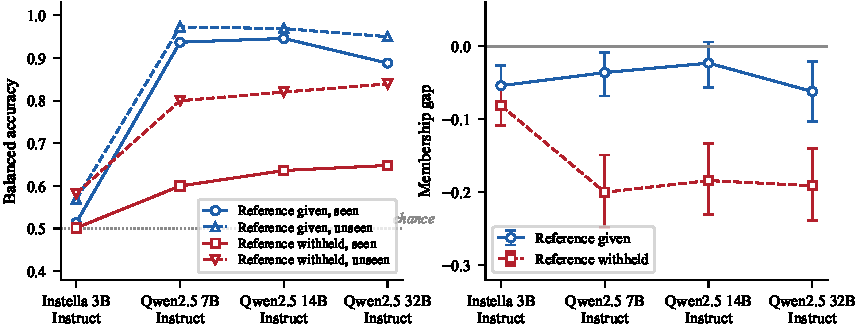
\includegraphics[width=\linewidth]{fig_ladder.pdf}
\caption{Left: absolute balanced accuracy for all four cells across the capability ladder.
Right: the membership gap with cluster bootstrap intervals. Capability lifts every series
and closes the control gap, leaving the reference free gap intact.}
\label{fig:ladder}
\end{figure}

\subsection{The failure is specificity, not sensitivity}
\label{sec:mech}

Balanced accuracy averages two rates that can move independently, and separating them
identifies the mechanism. Figure~\ref{fig:mech} decomposes both conditions. Sensitivity, the
rate of accepting correct solutions, carries no membership gap anywhere: $+0.011$
$[-0.005, +0.035]$ for Llama 3.1 8B and $-0.004$ $[-0.024, +0.016]$ for Qwen2.5 32B, both
spanning zero. Specificity, the rate of rejecting wrong solutions, collapses: $-0.496$
$[-0.572, -0.416]$ and $-0.378$ $[-0.471, -0.281]$ respectively. In absolute terms Llama 3.1
8B rejects 52.2 percent of wrong solutions to unseen problems and 2.7 percent of wrong
solutions to seen ones.

That asymmetry falsifies the account the design was originally built to test. A judge
comparing a candidate against a remembered answer would mark correct solutions wrong
whenever its memory were imperfect, producing a sensitivity loss. No such loss appears at
any judge in either condition. What appears instead is credulity: familiarity with a problem
raises the probability that a wrong solution to it is waved through.

\begin{figure}[t]
\centering
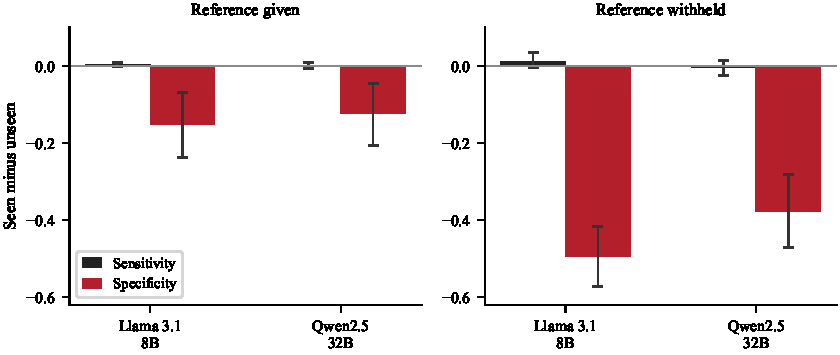
\includegraphics[width=\linewidth]{fig_mechanism.pdf}
\caption{Sensitivity and specificity gaps, seen minus unseen, under both conditions.
Sensitivity intervals contain zero everywhere. Specificity falls sharply once the reference
is withheld, which is the entire effect.}
\label{fig:mech}
\end{figure}

\subsection{Chance corrected agreement inflates the effect}

Cohen's kappa is the reflex choice for judge reliability and it misleads here.
Figure~\ref{fig:kappa} runs both statistics over one set of verdicts. With the reference
supplied the two agree to three decimals, both reporting $-0.074$. With it withheld, kappa
reports $-0.485$ where balanced accuracy reports $-0.243$, roughly double.

Nothing about agreement changed to produce that. Ground truth base rates are identical
across the two conditions, 0.772 on the seen arm against 0.526 on the unseen, because the
graded solutions do not change. What moves is the judge's own verdict marginal, and kappa
depends on both marginals as well as on agreement. An arm near one half carries more chance
corrected headroom than a skewed arm, so skew alone shifts the statistic. Feinstein and
Cicchetti~\citep{feinstein1990kappa} describe this as the first kappa paradox. The practical
consequence for evaluator reporting is narrow and concrete: where arms differ in base rate,
a chance corrected statistic will size a membership effect wrongly even when it points the
right way.

\begin{figure}[t]
\centering
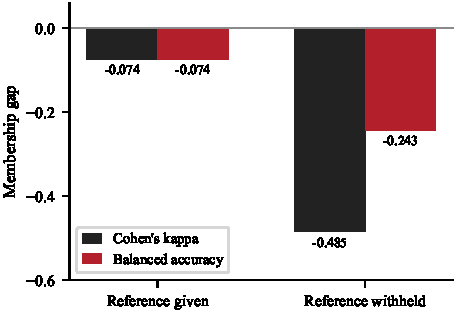
\includegraphics[width=0.46\linewidth]{fig_kappa.pdf}
\hfill
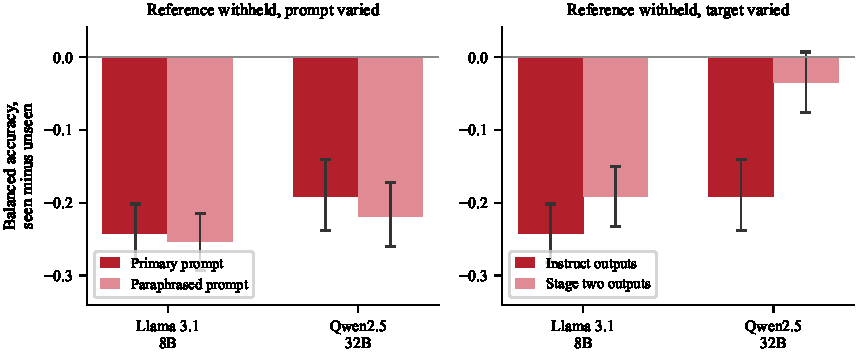
\includegraphics[width=0.52\linewidth]{fig_robustness.pdf}
\caption{Left: two statistics on identical verdicts for Llama 3.1 8B. They agree under the
control condition and diverge by a factor of two once the reference is withheld. Right: the
reference free gap under a paraphrased judging prompt and against a weaker generator.}
\label{fig:kappa}
\end{figure}

\subsection{Robustness}

Two explanations compete with the account above and both are testable.
Figure~\ref{fig:kappa} addresses them. A paraphrased judging prompt, rewritten to preserve
the task and change the wording, leaves the effect intact and slightly larger: $-0.254$
$[-0.293, -0.215]$ for Llama 3.1 8B against $-0.243$ with the primary prompt, and $-0.219$
$[-0.261, -0.172]$ for Qwen2.5 32B against $-0.191$. Prompt wording does not drive it.

Varying the generator does matter, and in the direction the account predicts. Grading the
weaker stage two checkpoint, whose errors are blunter, the strongest judge shows
$-0.035$ $[-0.077, +0.007]$, an interval containing zero, while Llama 3.1 8B on the same
target still shows $-0.192$ $[-0.232, -0.151]$. Errors coarse enough to catch without a
reference leave nothing for familiarity to erode, so the effect has a ceiling in how
gradeable the candidate solutions are.

\section{Implications for evaluator construct validity}

A judge is deployed as an instrument measuring solution correctness. The results above say
that instrument's specificity carries a term that depends on whether the graded item was in
its training corpus, and that the term is nearly invisible whenever a gold answer is
available. Benchmark practice makes this awkward, because the two conditions are not equally
common. Reference free grading is used precisely where no gold answer exists, on open ended
generation, on tasks scored by preference, and on new items for which references have not
been written. Those are the settings in which the measured degradation is largest.

The size is operationally relevant rather than marginal. A judge rejecting 52.2 percent of
wrong answers on unfamiliar problems and 2.7 percent on familiar ones is not applying one
standard with noise. It is applying two standards, and which one applies is determined by a
property of the judge's training data that the evaluation does not record and usually cannot
observe. Reporting balanced accuracy split by sensitivity and specificity, rather than a
single agreement number, makes the failure visible at low cost.

\section{Limitations}
\label{sec:limits}

\paragraph{Membership is verified for one judge, and it is not the judge carrying the
result.} Containment is measured against the Instella corpus, so the Instella judge has
verified membership but sits at chance. The Qwen and Llama judges show the effect and their
corpora are unknown, so for them the partition is GSM8K train against test rather than
verified seen against unseen. That asymmetry is why the primary claim is stated as a within
judge contrast between two conditions over identical items and identical candidate
solutions, which holds whatever the arm label means for a given judge. Closing the gap to a
membership claim requires a second open corpus model of comparable capability.

\paragraph{One family supplies the candidate solutions.} Every graded output comes from an
Instella checkpoint, and whether the dissociation reproduces on other generators is untested.
The judges span three families.

\paragraph{The effect has a ceiling in solution quality.} The stage two result above is
measured on one generator pair and should be treated as an observation rather than a law.

\paragraph{One checkpoint is unexplained.} Stage one outputs are wrong nearly everywhere and
trivially gradeable in either condition, which accounts for that null. The supervised fine
tuned checkpoint shows no gap in either condition despite output quality comparable to
instruct, and the present data do not explain why.

\paragraph{Attribution is not established.} No evidence links a verdict to a specific
training document. Section~\ref{sec:mech} narrows the effect to a specificity loss, which is
not attribution.

\section{Conclusion}

Measured against membership fixed by containment rather than estimated, an LLM judge shows a
small reliability loss on problems from its training corpus when the reference answer is
supplied, and a large one when it is withheld. The gap under reference free grading runs to
$-0.243$ in balanced accuracy and does not close with scale, while the same judges in the
control condition converge toward zero as they improve. The loss is entirely a specificity
failure, so familiarity buys credulity rather than confusion. Chance corrected agreement
roughly doubles the apparent effect on identical verdicts and should not be used to size it
where arms differ in base rate. The operational reading is specific: reference free grading
is the configuration deployed wherever no gold answer exists, and it is the configuration in
which the items most likely to sit in a judge's training data are graded least reliably.
